\chapter{PROPOSED SYSTEM}

\justify
This chapter details the architecture and protocol layout of our proposed 5G NR CU-DU split simulation. We will map the components of the disaggregated RAN, dissect the protocol stack from SDAP down to the physical layer, identify the target users, highlight the project's practical applications, and define the scope boundaries of our testbed.

\section{Description of Proposed System}
\justify
To model a split gNodeB deployment, we mapped the architectural options defined by 3GPP and chose Option 2 for the higher-layer split. Our simulation coordinates an end-to-end 5G Standalone network using the following components:

\begin{enumerate}[leftmargin=*]
    \item \textbf{5G Standalone Core Network (Open5GS):} Provides the network backbone with the following Network Functions:
    \begin{itemize}
        \item \textbf{NRF (NF Repository Function):} Acts as the service registry where all 5GC NFs register and discover each other via the SBI (Service-Based Interface). Configured at \texttt{127.0.0.10:7777}.
        \item \textbf{AMF (Access and Mobility Management Function):} Handles NAS signaling, UE authentication (5G-AKA), registration, and mobility management. Configured at \texttt{127.0.0.5} with NGAP listening for gNB connections. The AMF is configured with TAC=7 matching the RAN.
        \item \textbf{SMF (Session Management Function):} Manages PDU session establishment, modification, and release. Allocates UE IP addresses from the pool \texttt{10.45.0.0/16} for DNN ``internet''. Configured at \texttt{127.0.0.4}.
        \item \textbf{UPF (User Plane Function):} Routes and forwards user data packets between the DN (Data Network) and the gNB via GTP-U tunnels. GTP-U server at \texttt{127.0.0.20}. Session subnet \texttt{10.45.0.0/16}.
    \end{itemize}
    
    \item \textbf{gNB-CU (Centralized Unit -- OAI):} Centralizes RRC, PDCP, and SDAP layer processing. It connects to the AMF via the NG-C interface (NGAP/SCTP) and to the UPF via NG-U (GTP-U/UDP). It connects to both DUs via the F1 interface (F1AP/SCTP for control, GTP-U/UDP for user data) on port 2153. The CU also runs a Telnet server module on port 9091 for operator-triggered handover commands.
    
    \item \textbf{gNB-DU0 (Serving Cell):} Executes RLC, MAC, and PHY layer functions. Configured with Physical Cell ID (PCI) 0, NR Cell ID 12345678L, SSB frequency 630048 (3.45~GHz), and rfsimulator port 4043.
    
    \item \textbf{gNB-DU1 (Target Cell):} Configured with PCI 1, NR Cell ID 22222222L, SSB frequency 643296 (3.65~GHz), and rfsimulator port 4044.
    
    \item \textbf{Multi-Frequency UE (User Equipment -- OAI):} Emulates a mobile device with dual-RU sockets. Initially registers on DU0 and can switch to DU1 upon RRC reconfiguration.
\end{enumerate}

\begin{figure}[H]
\centering
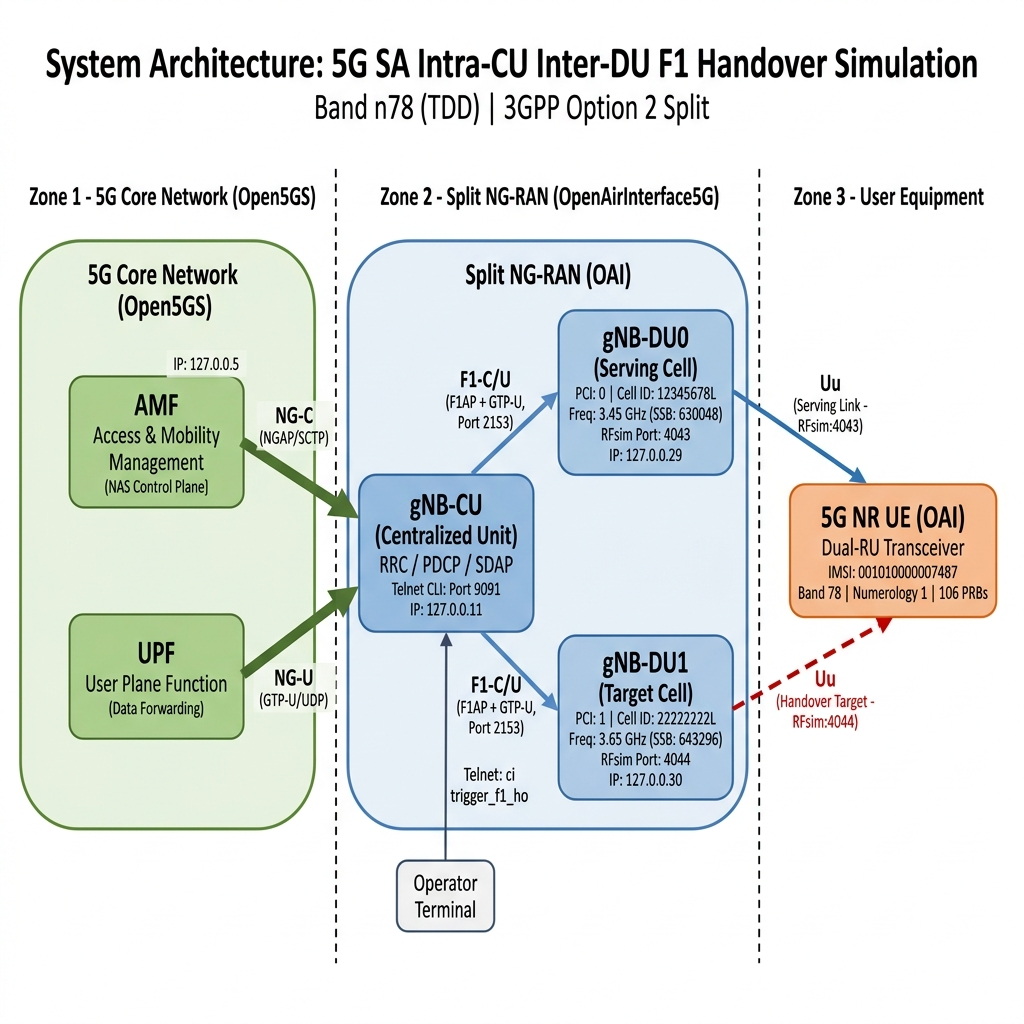
\includegraphics[width=0.95\textwidth]{images/system_architecture.png}
\caption{Complete System Architecture: 5G SA Intra-CU Inter-DU F1 Handover Simulation}
\label{fig:sys_arch}
\end{figure}

Figure \ref{fig:sys_arch} illustrates the complete network topology showing all nodes, their IP addresses, port bindings, carrier frequencies, and the protocol interfaces connecting them.


\section{Detailed Protocol Stack Description}
\justify
Understanding where layers are split is essential to understanding how the handover operates. In our Option 2 split design, the protocol layers are divided between the CU and the DU at the PDCP-RLC boundary, distributing the network logic as follows:

\begin{figure}[H]
\centering
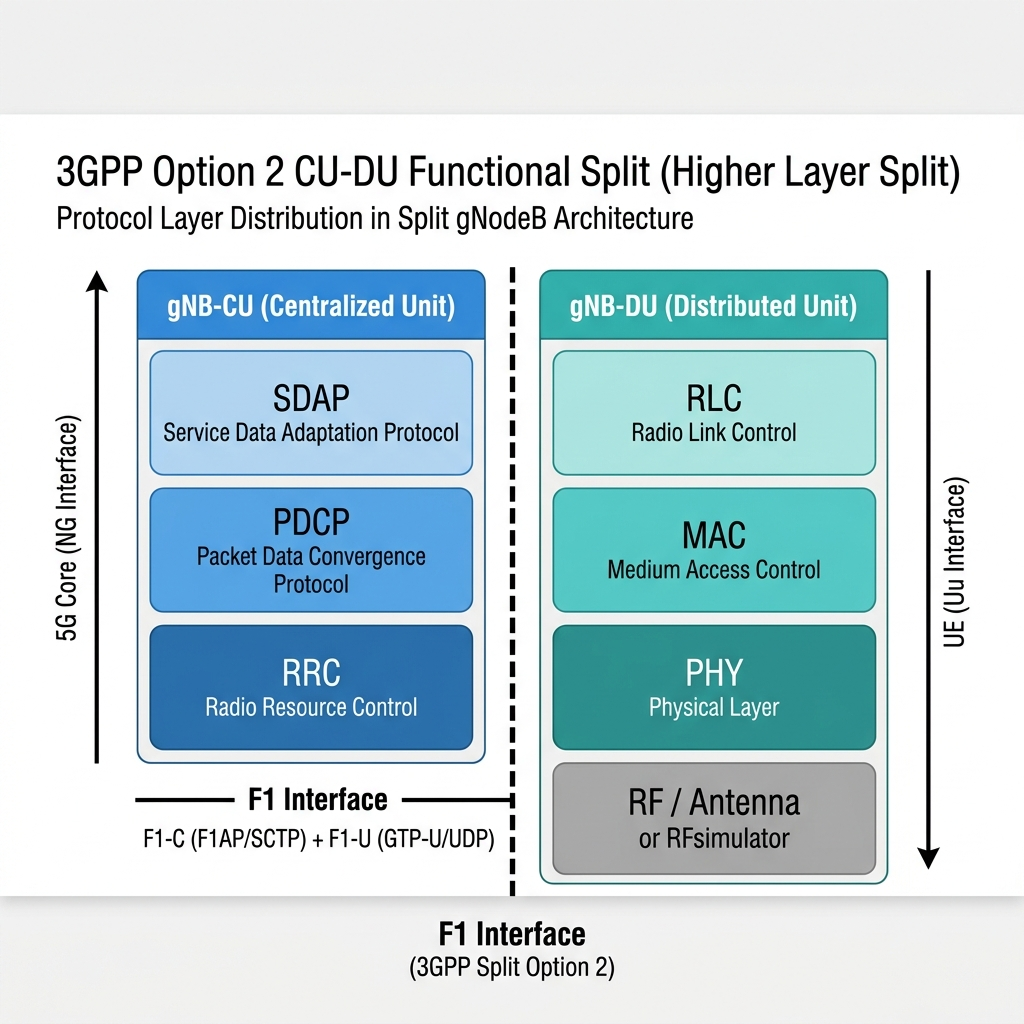
\includegraphics[width=0.85\textwidth]{images/protocol_stack_split.png}
\caption{3GPP Option~2 CU-DU Protocol Stack Split showing layer distribution}
\label{fig:proto_stack}
\end{figure}

Figure \ref{fig:proto_stack} shows the protocol layer distribution between the CU and DU. Each layer is described in detail below:

\subsection{Layers in the Centralized Unit (CU)}

\subsubsection{SDAP -- Service Data Adaptation Protocol}
The SDAP layer sits at the top of the user-plane stack in the CU. Its primary responsibilities are:
\begin{itemize}
    \item \textbf{QoS Flow to DRB Mapping:} SDAP maps Quality of Service (QoS) flows received from the 5G Core (via GTP-U tunnels from the UPF) to Data Radio Bearers (DRBs). Each QoS flow has a QoS Flow Identifier (QFI) that determines its treatment.
    \item \textbf{QoS Flow Marking:} SDAP marks uplink packets with their respective QFI so the UPF can apply correct forwarding policies.
    \item During handover, the SDAP mapping is maintained at the CU level, ensuring that QoS treatment is preserved regardless of which DU the UE is connected to.
\end{itemize}

\subsubsection{PDCP -- Packet Data Convergence Protocol}
The PDCP layer provides:
\begin{itemize}
    \item \textbf{Ciphering and Integrity Protection:} Encrypts user-plane data using algorithms like NEA0 (null ciphering in our simulation) and provides integrity protection using NIA2 (Snow3G-based) for control-plane SRBs (Signaling Radio Bearers).
    \item \textbf{Header Compression:} Uses ROHC (Robust Header Compression) to compress IP/UDP/RTP headers, reducing radio interface overhead.
    \item \textbf{Sequence Numbering:} Assigns PDCP sequence numbers (SNs) for in-order delivery and duplicate detection.
    \item \textbf{Data Recovery During Handover:} PDCP maintains a transmit buffer. During handover, unacknowledged PDCP PDUs from DU0 can be retransmitted to DU1, enabling lossless handover.
\end{itemize}

\subsubsection{RRC -- Radio Resource Control}
The RRC layer is the control-plane brain of the CU:
\begin{itemize}
    \item \textbf{Connection Management:} Manages UE states (RRC\_IDLE, RRC\_INACTIVE, RRC\_CONNECTED) and handles connection setup, reconfiguration, and release.
    \item \textbf{Measurement Configuration:} Configures the UE with measurement objects, report configurations, and measurement IDs for events like A2 (serving cell becomes weaker than threshold) and A3 (neighbour cell becomes offset better than serving).
    \item \textbf{Handover Execution:} Generates the \texttt{RRCReconfiguration} message containing the target cell's \texttt{CellGroupConfig} (frequency, PCI, RACH parameters), which instructs the UE to switch to the target DU.
    \item \textbf{Mobility Decision:} The CU's RRC entity makes the handover decision based on measurement reports or manual operator triggers, and coordinates with both source and target DUs via F1AP.
\end{itemize}

\subsection{Layers in the Distributed Unit (DU)}

\subsubsection{RLC -- Radio Link Control}
The RLC layer provides:
\begin{itemize}
    \item \textbf{Segmentation and Reassembly:} Segments PDCP PDUs received from the CU into RLC SDUs sized to fit into the MAC transport blocks, and reassembles them on the receiving side.
    \item \textbf{ARQ (Automatic Repeat Request):} In Acknowledged Mode (AM), RLC provides reliable delivery through retransmission of lost segments using STATUS PDUs.
    \item \textbf{Three Operating Modes:} Transparent Mode (TM) for broadcast, Unacknowledged Mode (UM) for delay-sensitive traffic, and Acknowledged Mode (AM) for reliable data transfer.
\end{itemize}

\subsubsection{MAC -- Medium Access Control}
The MAC layer is the scheduler and multiplexer:
\begin{itemize}
    \item \textbf{Scheduling:} Allocates physical resource blocks (PRBs) to UEs in both downlink and uplink directions based on channel quality indicators (CQI), buffer status reports (BSR), and QoS requirements.
    \item \textbf{HARQ (Hybrid ARQ):} Implements stop-and-wait HARQ with soft combining for rapid error correction at the physical layer.
    \item \textbf{Random Access (RACH):} Manages the Random Access Channel procedure (4-step RACH: Msg1 preamble, Msg2 RAR, Msg3 RRC Setup Request, Msg4 Contention Resolution). During handover, a dedicated (contention-free) RACH is used.
    \item \textbf{Multiplexing/Demultiplexing:} Combines data from multiple logical channels into transport blocks for transmission.
\end{itemize}

\subsubsection{PHY -- Physical Layer}
The PHY layer handles:
\begin{itemize}
    \item \textbf{OFDM Modulation:} Uses CP-OFDM (Cyclic Prefix OFDM) in downlink and DFT-s-OFDM or CP-OFDM in uplink, with subcarrier spacing of 30~kHz (numerology $\mu=1$).
    \item \textbf{Physical Channels:} Manages PDSCH (data DL), PUSCH (data UL), PDCCH (control DL), PUCCH (control UL), PRACH (random access), and PSS/SSS/PBCH (synchronization/broadcast).
    \item \textbf{Channel Coding:} Uses LDPC codes for data channels and Polar codes for control channels.
    \item \textbf{In our simulation:} The PHY layer is connected to the RFsimulator instead of real RF hardware. IQ samples are packaged into UDP packets and sent over the loopback interface.
\end{itemize}


\section{Description of Target Users}
\justify
Our testbed is designed as an accessible, high-fidelity platform targeting three primary user groups:
\begin{itemize}[leftmargin=*]
    \item \textbf{Telecommunication Researchers:} Studying handover latency, radio link monitoring, and RRC algorithms in disaggregated 5G networks.
    \item \textbf{Network Engineers:} Validating F1 interface configurations, neighbour list setups, and frequency planning before deploying real hardware.
    \item \textbf{Academic Students:} Gaining practical experience with 5G protocol stacks and core network integrations.
\end{itemize}

\section{Advantages and Applications}
\justify
By building a software-based split RAN testbed, we unlocked several architectural and educational advantages:
\begin{itemize}[leftmargin=*]
    \item \textbf{Local Mobility Handling:} The handover is resolved entirely within the gNB-CU, avoiding path switch signaling with the core network AMF/UPF, minimizing latency.
    \item \textbf{Cost-Effective Prototyping:} The RFsimulator eliminates the need for SDR hardware, enabling testing on a single workstation.
    \item \textbf{Advanced Protocol Debugging:} Detailed log traces across CU, DU, and UE, combined with Wireshark captures of F1AP and NGAP, enable in-depth protocol analysis.
    \item \textbf{Open RAN Alignment:} The CU-DU split architecture aligns with O-RAN Alliance specifications, making this framework relevant for Open RAN research.
\end{itemize}

\begin{figure}[H]
\centering
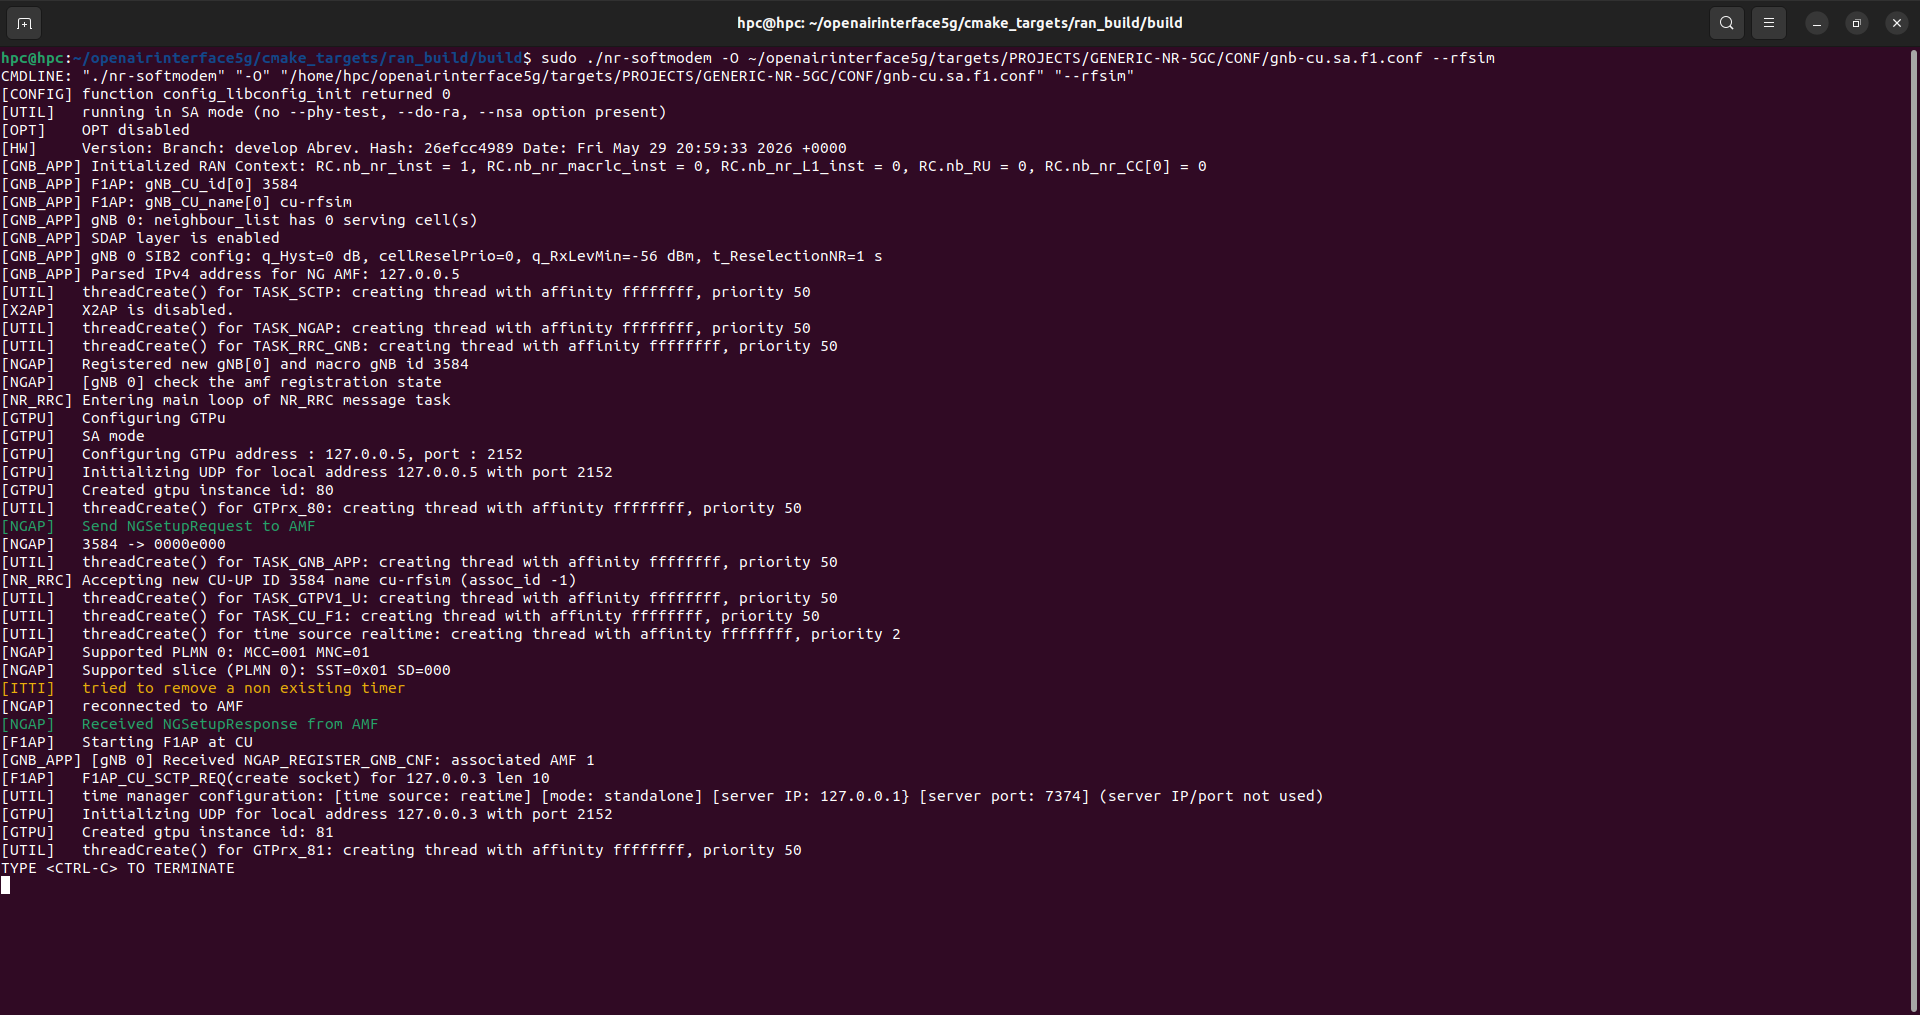
\includegraphics[width=0.85\textwidth]{images/core-cu_connection.png}
\caption{Core Network to CU active connection establishment logs}
\label{fig:core_cu}
\end{figure}

Figure \ref{fig:core_cu} shows the successful establishment of the NG interface between the CU and Open5GS core, confirming active transport layer bindings.


\section{Scope and Boundaries}
\justify
To keep our goals achievable while maintaining the technical depth of the study, we established clear boundaries for our testbed's scope:
\begin{itemize}[leftmargin=*]
    \item \textbf{In Scope:} Intra-CU inter-DU handover between cells controlled by a single gNB-CU; manual telnet-based handover trigger; single UE mobility analysis; protocol log verification.
    \item \textbf{Out of Scope:} Inter-CU handovers (Xn interface); core-assisted N2 handovers; multi-UE congestion testing; automated measurement-based handover triggers; real RF hardware deployment.
\end{itemize}